\chapter{Introduction} % Chapter title
\label{ch:intro}

Physical rehabilitation therapy allows people with a physical disability to recover and improve their quality of life. Those people might have suffered or may be at risk of suffering pain, injuries and disorders due to accidents, ageing or environmental and genetic factors \autocite{american2011today}. Physical rehabilitation therapy includes repetitions of a set of exercises, resulting in undesired effects on patients, such as a lack of motivation and condition worsening. Moreover, motivation is a key factor in physical rehabilitation since it may contribute to treatment completion \autocite{Shelton2015}. Thus, developing digital games for physical rehabilitation treatments has become relevant as a strategy to increase patients' motivation \autocite{Brokaw2015,Burke2009,Hernandez2013,McNeill2012,PirovanoAdvisor2012}. In this research work, those games are called \acp{PREG}.

On the other hand, \ac{PX} denotes the personal experience of of a player when playing digital games, thereby involving his/her subjective perceptions \autocite{Chu2011,Wiemeyer2016}. \ac{PX} is one of the most significant factors in determining the success of digital games in terms of fun, flow, enjoyment, engagement, satisfaction, pleasure and playability. Thus, evaluating \ac{PX} allows assessing if a \ac{PREG} increases patients’ motivation towards a therapy. 

\ac{PX} is a complex concept that involves different actors, such as context, game system and players \autocite{Engl2013,Fernandez2008,Nackea2}. Additionally, a \ac{PREG} should be evaluated considering motivational and therapeutic goals since it should provide a compelling experience to patients while assisting a physical rehabilitation treatment. Therefore, evaluators may consider limitations imposed by the rehabilitation context when evaluating \c{PX} in the context of \acp{PREG}. Previous works on evaluating \acp{PREG} have employed methods to evaluate conventional software and entertaining games, and some rehabilitation measurement instruments \autocite{Brokaw2015,Burke2009,jansen2013serious,Ni2014,Seo2016,Wuest2014}. However, there is no a standardised model to evaluate \ac{PX} in \acp{PREG}. Also, little is known about how the therapeutic goal of \acp{PREG} may affect \ac{PX} and its evaluation. Understanding the constraints that the therapeutic goal of \acp{PREG} may impose to \ac{PX} is important for evaluators to perform proper evaluations. In this research work, a \ac{PX} evaluation model for \acp{PREG} is proposed considering current research in \ac{PX} and a set of constraints of \acp{PREG}.

%----------------------------------------------------------------------------------------
\section{Problem Statement}

% Concentration in methods (how, when, which) (no aspects, no instruments) -> Integrative model
% criteria to select
% Evaluation based on evaluator xp
% when: planning evlaution and when comparing evaluations

\ac{PX} denotes the personal experience of playing digital games; thus, it involves a subjective perception of players \autocite{Wiemeyer2016,Chu2011}. Evaluating \ac{PX} consists in the observation and analysis of the interaction between players and games, applying methods from different fields, including usability, psychology, play testing \autocite{Wiemeyer2016}, gameplay metrics \autocite{Drachen2013} and physiological evaluation \autocite{Nacke2015}. A \ac{PX} evaluation might be useful to evaluate the effectiveness of a \ac{PREG} since it allows assessing aspects such as players' motivation, enjoyment or satisfaction. Therefore, \ac{PX} evaluation is a critical process to be included within the game development life cycle \autocite{Bernhaupt2015,McAllister2015,desurvire_methods_2013,Nacke2009}.

Additionally, \acp{PREG} have particular constraints imposed by the use of non-traditional devices (e.g., motion sensors) to enable interaction; the special needs of players/patients \autocite{Pirovano2016,Wiemeyer2015,Sinclair2007,Ni2014,Cameirao2010,Nijholt2008}; and the rehabilitation environment (e.g., physiotherapists may intervene during treatments) \autocite{Wiemeyer2015,Nijholt2008}. 

Nevertheless, there is no a general agreement about the \ac{PX} concept and how to evaluate it \autocite{Yanez-Gomez2017,Wiemeyer2016,Mueller2015}. Thus, \ac{PX} is evaluated based on evaluators experience and criteria, resulting in the difficulty to analyse and compare obtained results, and to replicate a certain evaluation. Also, evaluators may not consider the constraints of \acp{PREG} and concentrate on aspects such as motivation, enjoyment or usability \autocite{Brokaw2015,Ni2014,Cameirao2010,jansen2013serious}.

Therefore, the process of evaluating \ac{PX} in \acp{PREG} should be formalised. Accordingly, the research question to be addressed along this work is:

\begin{center} 
\emph{How can \ac{PX} evaluation be standardised in \acp{PREG}?}
\end{center} 

%----------------------------------------------------------------------------------------

%\section{Justification}\label{sec:problemJustfication}
% Comparative results
% evaluation planning objective

%The purpose of digital games is to provide a fun and engaging experience to players \autocite{Moosajee,Zammitto2014}. Meanwhile, serious games should provide a positive experience while achieving an additional goal; e.g., to train, educate or support a certain process \autocite{Wiemeyer2016}. Therefore, evaluating \ac{PX} has become a crucial process to be integrated along the game development life cycle since it allows assessing the effectiveness of a game to provide the expected experience \autocite{Bernhaupt2015,McAllister2015,desurvire_methods_2013,Nacke2009}. In this context, research fields like \ac{GUR} have evolved in the past years. \ac{GUR} encompasses concepts, methods, tools and techniques aimed to reach an optimal quality of \ac{PX}; i.e., create more compelling gameplay experiences \autocite{Moosajee,Nacke2015,Wiemeyer2016,Drachen2013}.

%An integral evaluation of \acp{PREG} should consider particular constraints. These constraints are mainly related to the use of motion sensors as mean of interaction \autocite{Wiemeyer2015,Nijholt2008} and the involved rehabilitation purpose. The effectiveness of a \ac{PREG} may be evaluated in terms of its capability to motivate patients and assist their rehabilitation therapy. A model for evaluating \ac{PX} in \acp{PREG} may contribute to address the lack of standardisation of this process and may be employed as a tool for validating the effectiveness objectively, guiding evaluators while performing an evaluation.

\section{Objectives}\label{sec:objectives}

%------------------------------------------------
\subsection{General Objective} 
Develop a \ac{PX} evaluation model for rehabilitation exergames.

%------------------------------------------------
\subsection{Specific Objectives}
\begin{enumerate}
\item Identify characteristics of rehabilitation exergames.
\item Define a set of aspects to be validated during a \ac{PX} evaluation in rehabilitation exergames.
\item Design a standard to create \ac{PX} evaluation questionnaires for rehabilitation exergames.
\item Design a procedure for \ac{PX} evaluation in rehabilitation exergames.
\item Design a model of \ac{PX} evaluation in rehabilitation exergames integrating identified characteristics, aspects, questionnaires standard and procedure.
\item Validate the model using a rehabilitation exergame.
\end{enumerate}
%------------------------------------------------
\subsection{Results and contributions}

The results of this research work are: 

\begin{itemize}
    \item A definition of \acp{PREG} and the identification of a set of properties to characterise a \acp{PREG}.
    \item The identification of a set of constraints to be considered when evaluating \ac{PX} in \acp{PREG}.
    \item The identification of relevant aspects, instruments and methods to evaluate \acp{PREG}.
    \item A standard to develop questionnaires to evaluate \ac{PX}.
    \item A questionnaire to assess physiotherapists perception regarding the use of a \ac{PREG}.
    \item A model to evaluate \ac{PX} in \acp{PREG}.
    \item A web application to use the proposed model.
    \item The evaluation of Playtherapy, a \ac{PREG} to be used at a local hospital.
    \item Two research papers that socialise the results of the conducted evaluation. Both awarded in the conferences in which were presented.
\end{itemize}

Additionally, during the development of this research work, six undergraduate students who participated in the development of Playtherapy were advised as part of their final degree projects.


%----------------------------------------------------------------------------------------
\section{Structure of the document}

This document presents the development of a \ac{PX} evaluation model for \acp{PREG}. An overview of the document is presented in \autoref{fig:documentOverview}.

\begin{figure}[htb]
\myfloatalign
{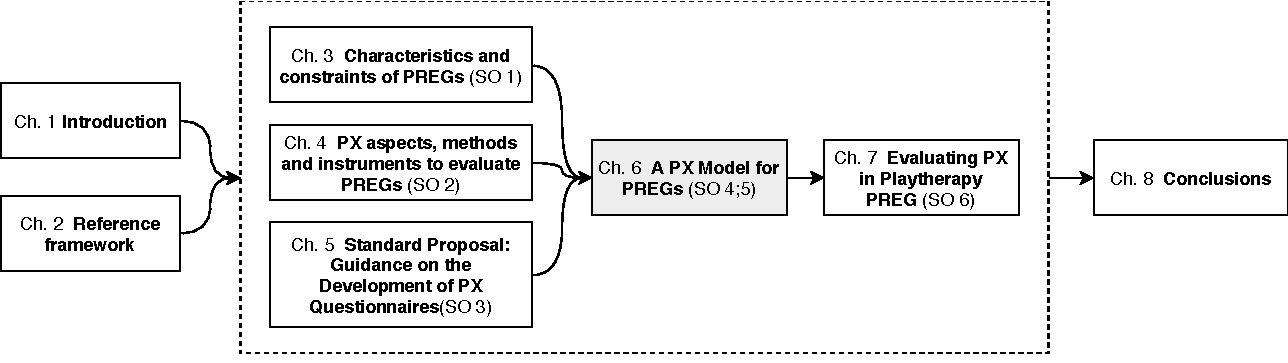
\includegraphics[width=\linewidth]{gfx/intro/documentOverview}} \quad
\caption{Overview of the document and relation between chapters (CH) and specific objectives (SO)}\label{fig:documentOverview}
\end{figure}

The remaining of the document is organised as follows: first, \autoref{ch:referenceFramework} presents the reference framework of the work and the state of the art of the \ac{PX} research field. After that, \autoref{ch:characterising} presents a qualitative study conducted to identify characteristics, constraints and an approach to characterise \acp{PREG} regarding \ac{PX}. Then, \autoref{ch:aspects} describes relevant aspects, methods and instruments to evaluate \ac{PX} in \acp{PREG} and the identification process that we carried out. After that, a comprehensive \ac{PX} model for evaluating \acp{PREG} is proposed in \autoref{ch:model}. Additionally, a methodology to evaluate \ac{PX} in \acp{PREG} based on the proposed model is presented in this section. Then, \autoref{ch:questionnaire} presents a standard proposal to develop \ac{PX} evaluation questionnaires and a questionnaire to assess physiotherapists' perception of \ac{PREG}. \autoref{ch:playtherapy} presents a case study in which the findings of this research work were employed to evaluate a \ac{PREG} developed by the Multimedia and Vision research group from \textit{Universidad del Valle} and Evaristo Garc\'ia University Hospital in Cali Colombia. Finally, we summarise and conclude the results of this research work in \autoref{ch:conclusions}.